% !TeX program = xelatex
\documentclass{article}
\usepackage{kotex}
\usepackage[a4paper,left=3cm, right=3cm, top=2cm, bottom=2cm]{geometry}
\usepackage{amsmath}
\usepackage{graphicx}
\usepackage{caption}
\usepackage{setspace}
\usepackage{xcolor}
\usepackage{titlesec}
\usepackage{amssymb}
\usepackage{tcolorbox}
\usepackage{wrapfig}
\usepackage{amsthm}
\usepackage{multirow}
\usepackage{array}
\usepackage{tikz}
\usetikzlibrary{positioning,arrows.meta,matrix}
\usepackage{longtable}
\usepackage{pgfplots}
\pgfplotsset{compat=1.18}

\title{2.1 Determinants by Cofactor Expansion}
\date{}
\author{}
\setstretch{1.3}

\titleformat{name=\section, numberless}
  {\normalfont\large\bfseries\color{blue}}
  {}
  {0pt}
  {}
\geometry{a4paper, margin=1in}

\newcommand{\redheading}[1]{{\vspace{2mm}\noindent\Large\bfseries\color{red!55!black} #1\par}\vspace{2mm}}

\newtheoremstyle{mystyle}
  {}{}{\itshape}{}{\bfseries}{.}{.5em}{}
\theoremstyle{mystyle}

\begin{document}
\maketitle

% Chapter 2 overview
\begin{tcolorbox}[colback=blue!5, colframe=blue!60!black,
  title={\textbf{Chapter 2: Determinants}}, boxrule=0.5mm, arc=3mm]
\textbf{Chapter Contents:}
\textbf{Introduction.} Determinant functions assign a real number $f(A)$ to a matrix $A$. Although they arose in the context of linear systems, their main value is linking together the major concepts of linear algebra and providing a formula for the matrix inverse.
\end{tcolorbox}

\vspace{3mm}
{\itshape\color{blue!45!black}
In this section we define the notion of a ``determinant.'' This enables a specific formula for the inverse of an invertible matrix and, in turn, a formula for solutions of certain kinds of linear systems.\par}

\vspace{2mm}

Recall from Theorem 1.4.5 that the $2\times 2$ matrix $A=\begin{bmatrix}a&b\\c&d\end{bmatrix}$ is invertible iff $ad-bc\neq0$; $ad-bc$ is the \textbf{determinant} of $A$:
\[
\det(A)=ad-bc\quad\text{or}\quad\begin{vmatrix}a&b\\c&d\end{vmatrix}=ad-bc \tag{1}
\]
and the inverse is
\[
A^{-1}=\frac{1}{\det(A)}\begin{bmatrix}d&-b\\-c&a\end{bmatrix} \tag{2}
\]

\redheading{Minors and Cofactors}

To extend Formula (2) to square matrices of all orders, we use subscripted entries. For a $2\times2$ matrix $A=[a_{ij}]$:
\[
\det(A)=\begin{vmatrix}a_{11}&a_{12}\\a_{21}&a_{22}\end{vmatrix}=a_{11}a_{22}-a_{12}a_{21} \tag{3}
\]
Writing the same in a form that also works as
\[
\det\begin{bmatrix}a_{11}&a_{12}\\a_{21}&a_{22}\end{bmatrix}=\det[a_{11}]\det[a_{22}]-\det[a_{12}]\det[a_{21}] \tag{4}
\]
where $\det[a_{11}]=a_{11}$ for a $1\times1$ matrix. This inductive pattern extends: a $3\times3$ determinant is defined via $2\times2$ determinants, a $4\times4$ via $3\times3$, and so on.

\begin{tcolorbox}[colback=teal!4, colframe=teal!65!black,
  title={\textbf{Definition 1}}, boxrule=0.5mm, arc=3mm]
If $A$ is a square matrix, the \textbf{minor of entry $a_{ij}$}, denoted $M_{ij}$, is the determinant of the submatrix obtained by deleting the $i$th row and $j$th column of $A$. The \textbf{cofactor of entry $a_{ij}$} is
\[
C_{ij}=(-1)^{i+j}M_{ij}
\]
\end{tcolorbox}

\subsection*{EXAMPLE 1 | Finding Minors and Cofactors}
Let $A=\begin{bmatrix}3&1&-4\\2&5&6\\1&4&8\end{bmatrix}$.

\textbf{SOLUTION:} The minor of $a_{11}$ is obtained by deleting row 1 and column 1:
\[
M_{11}=\begin{vmatrix}5&6\\4&8\end{vmatrix}=40-24=16 \implies C_{11}=(-1)^{1+1}M_{11}=16
\]
The minor of $a_{32}$ is obtained by deleting row 3 and column 2:
\[
M_{32}=\begin{vmatrix}3&-4\\2&6\end{vmatrix}=18-(-8)=26 \implies C_{32}=(-1)^{3+2}M_{32}=-26
\]

\textbf{Remark.} The sign $(-1)^{i+j}$ follows the checkerboard pattern
\[
\begin{bmatrix}+&-&+&-&\cdots\\-&+&-&+&\cdots\\+&-&+&-&\cdots\\\vdots&\vdots&\vdots&\vdots&\ddots\end{bmatrix}
\]
so $C_{11}=M_{11}$, $C_{21}=-M_{21}$, $C_{22}=M_{22}$, etc. In practice, compute $M_{ij}$ and adjust the sign by the pattern.

\subsection*{EXAMPLE 2 | Cofactor Expansions of a $2\times2$ Matrix}
For $A=[a_{ij}]$, $\det(A)=\begin{vmatrix}a_{11}&a_{12}\\a_{21}&a_{22}\end{vmatrix}$ can be written four ways using cofactors:
\begin{align*}
&= a_{11}C_{11}+a_{12}C_{12} &&\text{(row 1)}\\
&= a_{21}C_{21}+a_{22}C_{22} &&\text{(row 2)}\\
&= a_{11}C_{11}+a_{21}C_{21} &&\text{(column 1)}\\
&= a_{12}C_{12}+a_{22}C_{22} &&\text{(column 2)} \tag{6}
\end{align*}
Each sum is a \textbf{cofactor expansion}: entries and cofactors from the same row or column.

\vspace{2mm}

This generalizes to matrices of any order:

\begin{tcolorbox}[colback=red!4, colframe=red!60!black,
  title={\textbf{Theorem 2.1.1}}, boxrule=0.5mm, arc=3mm]
If $A$ is an $n\times n$ matrix, then regardless of which row or column is chosen, the number obtained by multiplying the entries in that row (or column) by their cofactors and summing is always the same.
\end{tcolorbox}

This allows the following definition.

\begin{tcolorbox}[colback=teal!4, colframe=teal!65!black,
  title={\textbf{Definition 2}}, boxrule=0.5mm, arc=3mm]
If $A$ is an $n\times n$ matrix, then $\det(A)$ is defined by the \textbf{cofactor expansions}:
\begin{align*}
\det(A)&=a_{1j}C_{1j}+a_{2j}C_{2j}+\cdots+a_{nj}C_{nj} &&\text{[along the }j\text{th column]} \tag{7}\\
\det(A)&=a_{i1}C_{i1}+a_{i2}C_{i2}+\cdots+a_{in}C_{in} &&\text{[along the }i\text{th row]} \tag{8}
\end{align*}
\end{tcolorbox}

\subsection*{EXAMPLE 3 | Cofactor Expansion Along the First Row}
Find $\det(A)$ for $A=\begin{bmatrix}3&1&0\\-2&-4&3\\5&4&-2\end{bmatrix}$.

\textbf{SOLUTION:}
\begin{align*}
\det(A)&=3\begin{vmatrix}-4&3\\4&-2\end{vmatrix}-1\begin{vmatrix}-2&3\\5&-2\end{vmatrix}+0\begin{vmatrix}-2&-4\\5&4\end{vmatrix}\\
&=3(8-12)-1(4-15)+0\\
&=3(-4)-1(-11)=-12+11=\boxed{-1}
\end{align*}

\subsection*{EXAMPLE 4 | Cofactor Expansion Along the First Column}
Using the same $A$ as Example 3, expand along column 1.

\textbf{SOLUTION:}
\begin{align*}
\det(A)&=3\begin{vmatrix}-4&3\\4&-2\end{vmatrix}-(-2)\begin{vmatrix}1&0\\4&-2\end{vmatrix}+5\begin{vmatrix}1&0\\-4&3\end{vmatrix}\\
&=3(-4)-(-2)(-2)+5(3)\\
&=-12-4+15=\boxed{-1}
\end{align*}

\subsection*{EXAMPLE 5 | Smart Choice of Row or Column}
If $A=\begin{bmatrix}1&0&0&-1\\3&1&2&2\\1&0&-2&1\\2&0&0&1\end{bmatrix}$, find $\det(A)$.

\textbf{SOLUTION:} Column 2 has three zeros, so expand along it:
\[
\det(A)=1\cdot C_{22}=1\cdot\begin{vmatrix}1&0&-1\\1&-2&1\\2&0&1\end{vmatrix}
\]
For the resulting $3\times3$, column 2 again has two zeros; expand along it:
\[
\begin{vmatrix}1&0&-1\\1&-2&1\\2&0&1\end{vmatrix}=(1)(-2)\begin{vmatrix}1&-1\\2&1\end{vmatrix}=-2(1+2)=-6
\]
Therefore $\det(A)=1\cdot(-6)=\boxed{-6}$.

\subsection*{EXAMPLE 6 | Determinant of a Lower Triangular Matrix}
The determinant of a $4\times4$ lower triangular matrix equals the product of its diagonal entries:
\[
\begin{vmatrix}a_{11}&0&0&0\\a_{21}&a_{22}&0&0\\a_{31}&a_{32}&a_{33}&0\\a_{41}&a_{42}&a_{43}&a_{44}\end{vmatrix}
=a_{11}\begin{vmatrix}a_{22}&0&0\\a_{32}&a_{33}&0\\a_{42}&a_{43}&a_{44}\end{vmatrix}
=a_{11}a_{22}\begin{vmatrix}a_{33}&0\\a_{43}&a_{44}\end{vmatrix}
=a_{11}a_{22}a_{33}a_{44}
\]
(Expand along the first row at each step; only the $(1,1)$ entry is nonzero.)

\begin{tcolorbox}[colback=red!4, colframe=red!60!black,
  title={\textbf{Theorem 2.1.2}}, boxrule=0.5mm, arc=3mm]
If $A$ is an $n\times n$ triangular matrix (upper, lower, or diagonal), then
\[
\det(A)=a_{11}a_{22}\cdots a_{nn}
\]
\end{tcolorbox}

\redheading{A Useful Technique for Evaluating $2\times2$ and $3\times3$ Determinants}

For $2\times2$ matrices, $\det(A)$ equals the product of entries on the rightward diagonal minus the product on the leftward diagonal. For $3\times3$ matrices, recopy the first two columns to the right; sum the three rightward diagonal products and subtract the three leftward diagonal products.

\begin{center}
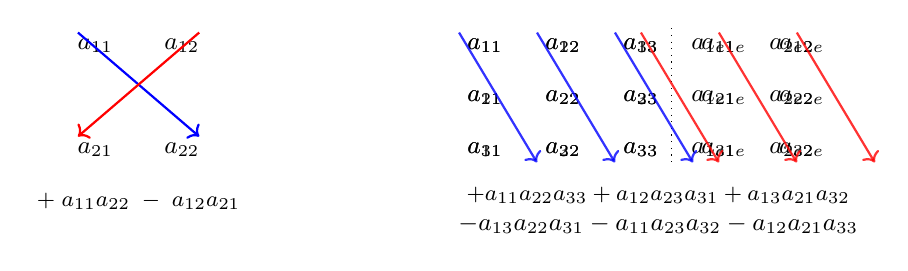
\begin{tikzpicture}[scale=1.1, every node/.style={font=\small}]
% --- 2x2 block ---
\node (a11) at (0,1.2) {$a_{11}$};
\node (a12) at (1.0,1.2) {$a_{12}$};
\node (a21) at (0,0) {$a_{21}$};
\node (a22) at (1.0,0) {$a_{22}$};
% positive diagonal (right arrow)
\draw[->,blue,thick] (-0.2,1.35) -- (1.2,0.15);
% negative diagonal (left arrow)
\draw[->,red,thick] (1.2,1.35) -- (-0.2,0.15);
\node at (0.5,-0.6) {\footnotesize $+\;a_{11}a_{22}\;-\;a_{12}a_{21}$};

% --- 3x3 block (with 2 extra columns) ---
\begin{scope}[xshift=4.5cm]
\foreach \r/\lab in {1.2/1, 0.6/2, 0/3}{
  \foreach \c/\lab in {0/1,0.9/2,1.8/3,2.7/1e,3.6/2e}{
    \node at (\c,\r) {$a_{\lab\lab}$};
  }
}
% Overwrite repeated column labels
\node at (0,1.2) {$a_{11}$}; \node at (0.9,1.2) {$a_{12}$}; \node at (1.8,1.2) {$a_{13}$};
\node at (0,0.6) {$a_{21}$}; \node at (0.9,0.6) {$a_{22}$}; \node at (1.8,0.6) {$a_{23}$};
\node at (0,0)   {$a_{31}$}; \node at (0.9,0)   {$a_{32}$}; \node at (1.8,0)   {$a_{33}$};
\node at (2.7,1.2) {$a_{11}$}; \node at (3.6,1.2) {$a_{12}$};
\node at (2.7,0.6) {$a_{21}$}; \node at (3.6,0.6) {$a_{22}$};
\node at (2.7,0)   {$a_{31}$}; \node at (3.6,0)   {$a_{32}$};
% vertical divider
\draw[dotted] (2.15,1.4)--(2.15,-0.2);
% 3 positive diagonals (blue)
\draw[->,blue,thick,opacity=0.8] (-0.3,1.35)  -- (0.6,-0.15);
\draw[->,blue,thick,opacity=0.8] (0.6,1.35)   -- (1.5,-0.15);
\draw[->,blue,thick,opacity=0.8] (1.5,1.35)   -- (2.4,-0.15);
% 3 negative diagonals (red)
\draw[->,red,thick,opacity=0.8]  (1.8,1.35)   -- (2.7,-0.15);
\draw[->,red,thick,opacity=0.8]  (2.7,1.35)   -- (3.6,-0.15);
\draw[->,red,thick,opacity=0.8]  (3.6,1.35)   -- (4.5,-0.15);
\end{scope}

\node[align=center] at (6.5,-0.7) {\footnotesize $+a_{11}a_{22}a_{33}+a_{12}a_{23}a_{31}+a_{13}a_{21}a_{32}$\\$-a_{13}a_{22}a_{31}-a_{11}a_{23}a_{32}-a_{12}a_{21}a_{33}$};
\end{tikzpicture}
\end{center}

\textbf{Warning.} The arrow technique works \emph{only} for $2\times2$ and $3\times3$ determinants; it does \emph{not} generalize to $4\times4$ or higher.

\subsection*{EXAMPLE 7 | A Technique for Evaluating $2\times2$ and $3\times3$ Determinants}

\textbf{SOLUTION:}
\[
\begin{vmatrix}3&1\\4&-2\end{vmatrix}=(3)(-2)-(1)(4)=-10
\]
\[
\begin{vmatrix}1&2&3\\-4&5&6\\7&-8&9\end{vmatrix}
=\bigl[45+84+96\bigr]-\bigl[105-48-72\bigr]=225-(-15)=\boxed{240}
\]
(Rightward products: $1\cdot5\cdot9=45$, $2\cdot6\cdot7=84$, $3\cdot(-4)\cdot(-8)=96$;
leftward products: $3\cdot5\cdot7=105$, $1\cdot6\cdot(-8)=-48$, $2\cdot(-4)\cdot9=-72$.)

\section*{Exercise Set 2.1}

\begin{enumerate}

\item[1.] Find all minors and cofactors of
$A=\begin{bmatrix}1&-2&3\\6&7&-1\\-3&1&4\end{bmatrix}$.

\item[3.] Let $A=\begin{bmatrix}4&-1&1&6\\0&0&-3&3\\4&1&0&14\\4&1&3&2\end{bmatrix}$. Find:
(a) $M_{13}$ and $C_{13}$\quad (b) $M_{23}$ and $C_{23}$\quad
(c) $M_{22}$ and $C_{22}$\quad (d) $M_{21}$ and $C_{21}$

\item[5.] Evaluate $\det(A)=\begin{vmatrix}3&5\\-2&4\end{vmatrix}$. If $A$ is invertible, find $A^{-1}$ using Formula (2).

\item[7.] Evaluate $\det(A)=\begin{vmatrix}-5&7\\-7&-2\end{vmatrix}$. If $A$ is invertible, find $A^{-1}$.

\noindent\textit{In Exercises 9--11, use the arrow technique to evaluate the determinant.}

\item[9.] $\begin{vmatrix}a-3&5\\-3&a-2\end{vmatrix}$

\item[11.] $\begin{vmatrix}-2&1&4\\3&5&-7\\1&6&2\end{vmatrix}$

\noindent\textit{In Exercises 15--17, find all values of $\lambda$ for which $\det(A)=0$.}

\item[15.] $A=\begin{bmatrix}\lambda-2&1\\-5&\lambda+4\end{bmatrix}$

\item[17.] $A=\begin{bmatrix}\lambda-1&0\\2&\lambda+1\end{bmatrix}$

\item[19.] Evaluate the determinant of the matrix in Exercise 13,
$A=\begin{bmatrix}3&0&0\\2&-1&5\\1&9&-4\end{bmatrix}$,
by cofactor expansion along: (a) the first row,\; (b) the first column,\;
(c) the second row,\; (d) the second column,\; (e) the third row,\; (f) the third column.

\noindent\textit{In Exercises 21--25, evaluate $\det(A)$ by cofactor expansion along a row or column of your choice.}

\item[21.] $A=\begin{bmatrix}-3&0&7\\2&5&1\\-1&0&5\end{bmatrix}$

\item[24.] $A=\begin{bmatrix}k+1&k-1&7\\2&k-3&4\\5&k+1&k\end{bmatrix}$

\item[25.] $A=\begin{bmatrix}3&3&0&5\\2&2&0&-2\\4&1&-3&0\\2&10&3&2\end{bmatrix}$

\noindent\textit{In Exercises 27--32, evaluate $\det(A)$ by inspection.}

\item[27.] $A=\begin{bmatrix}1&0&0\\0&-1&0\\0&0&1\end{bmatrix}$

\item[30.] $A=\begin{bmatrix}1&1&1&1\\0&2&2&2\\0&0&3&3\\0&0&0&4\end{bmatrix}$

\item[32.] $A=\begin{bmatrix}-3&0&0&0\\1&2&0&0\\40&10&-1&0\\100&200&-23&3\end{bmatrix}$

\item[33.] In each part, show that the value of the determinant is independent of $\theta$.
\begin{enumerate}
  \item[(a)] $\begin{vmatrix}\sin\theta&\cos\theta\\-\cos\theta&\sin\theta\end{vmatrix}$
  \item[(b)] $\begin{vmatrix}\sin\theta&\cos\theta&0\\-\cos\theta&\sin\theta&0\\\sin\theta-\cos\theta&\sin\theta+\cos\theta&1\end{vmatrix}$
\end{enumerate}

\item[36.] Show that $\det(A)=\dfrac{1}{2}\begin{vmatrix}\operatorname{tr}(A)&1\\\operatorname{tr}(A^2)&\operatorname{tr}(A)\end{vmatrix}$ for every $2\times2$ matrix $A$.

\item[37.] What can you say about an $n$th-order determinant all of whose entries are 1? Explain.

\item[38.] What is the maximum number of zeros that a $3\times3$ matrix can have without having a zero determinant? Explain.

\noindent\textbf{Working with Proofs}

\item[40.] Prove that $(x_1,y_1)$, $(x_2,y_2)$, $(x_3,y_3)$ are collinear if and only if
$\begin{vmatrix}x_1&y_1&1\\x_2&y_2&1\\x_3&y_3&1\end{vmatrix}=0$.

\item[43.] A matrix of the form $V=\begin{bmatrix}1&a&a^2\\1&b&b^2\\1&c&c^2\end{bmatrix}$ (and its higher-order analogs) is called a \textbf{Vandermonde matrix}. Use cofactor expansion to prove that
\[
\begin{vmatrix}1&x_1&x_1^2\\1&x_2&x_2^2\\1&x_3&x_3^2\end{vmatrix}=(x_2-x_1)(x_3-x_1)(x_3-x_2)
\]

\end{enumerate}

\end{document}
